\chapter{Introduction}
\label{chp:intro}

\section{Motivation}
\par Based on existing access control system, it is quite promising idea about making normal user have control of the residential area internet access control by using smart filtering, informing and time management. Since the smart phone with the mobile internet access functionality released, more and more sociology research, for instance the paper form Jim McGuigan\cite{MobilePhoneSociology}, show that there are many weakness of over using mobile phone and internet. The idea of this project is to  meet the need of the people who would like to control the daily use of the internet and manager other people access right to some specific wireless network.
\par Nowadays people are using smart phone to do as much task as they can, because smart phone is easy to carry with and smart phone is the only necessary access people need to have the tons of internet information. Then the requirement of using smart phone to control the existing daily life system such as wireless router, switch and other electronic devices are growing rapidly. This prototype project is to fill the missing part of the previous project to connect the access control system to \gls{ios} devices. There are static article\cite{MobileOSMarketShare} shows that Android has 81.0 percent smartphone share in the third quarter of 2013  and \gls{ios} has 12.9 percent, these two mobile operating system shared most mobile operating system in the world. This project will focus on the \gls{ios} application to work with the improved access control system. It will make the whole system become more user friendly for normal user to choose different mobile operating system to administrate the system.

\section{Related Work}
\par There are many security software can do internet control in the market. Such as Norton Family application\cite{Norton}, K9 web Protection\cite{K9}, OpenDNS\cite{OpenDNS} and etc. Most of them can provide block web sites, time restrictions, easy log reports of internet activity and etc. But these kind of software need to install in every access device in the network. And also it could be uninstalled and broken by accident. They are more like voluntarily joining the internet control policy, which is used greatly on parent and children case but no more other normal cases.
\par There is a kickstarter\cite{kickstarterCircle} project which has the similar idea as this prototype project. The product name is 'Circle'\cite{Circle}.Circle is a device\ref{fig:circle_project}, managed by an \gls{ios} app, that enables user to choose how you and your family spend time online by using advanced filtering, time management systems and informing to answer the where,why,and how of your network's internet activity. Although it is just a start-up project, its concept and prototype device are quite promising in the promote video on the kickstarter. The main and unique functionalities Circle has are time management capabilities, device and application notifications, safe,pause and bedtime modes and cost effective for the system. 
\begin{figure}
	\centering
    	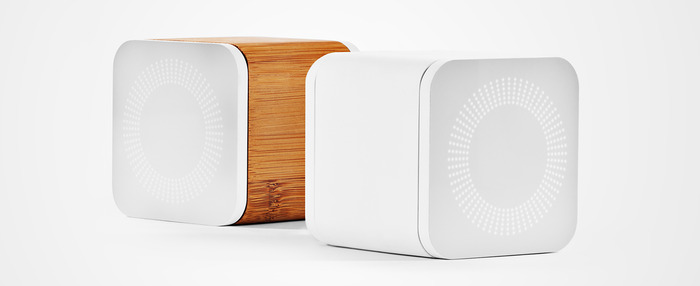
\includegraphics[width=0.90\textwidth]{figs/circleDevice.jpg}
  	\caption{Kickstarter Project: Meet Circle}
  	\label{fig:circle_project}
\end{figure}
\par The prototype of this report is using \gls{rpi} as the same function as Circle's wireless router. And this prototype system has server side back-end to store client and administrator user database. There are android and \gls{ios} applications both work with the internet control system in this project.
\par At application side, the prototype application of this report will have the same administrator function to approve and block the client internet access request through http request.
\par For the notification function of the system, the project of this report has the similar idea with another kickstarter project 'NINJA SPHERE'\cite{ninja_sphere}. The idea of NINJA SPHERE is to make the next generation control of your environment with accurate in-home location data and a gesture control interface. Although the project of this report will not cover the advanced way to control the environment of the residential area only the internet access control of the residential area, the idea is still the same to use mobile application to communicate with the other device and even get notification from other device in the same wireless network area. 
\par The notification of the client request in this project will be sent as notification E-mail. It makes the administrator get updated request information from the internet access control system.

\section{Scope}
\par The first part of this project will be using the \gls{rpi} device and the code script from previous student master project report\cite{TorgeirMR} and previous student Github repository\cite{TorgierGit} to set up the internet access control system working.Because the \gls{rpi} device and \gls{sd} card  got from the previous student are without any code and configuration, they should be configured with the reference of previous student master project report.
\par The second part of this project will be setting up the central management server on the test domain 'apc.item.ntnu.no'(129.241.200.170)  from \gls{item} department of \gls{ntnu}. The work of this report will cover some security concern improvement and some new notification mechanism implement on the remote central management server.And the database structure of the system stored on the remote server would be changed according to the new functionality of the improved internet access control system.
\par The third part of this project will be implementation of the \gls{ios} application intended for end-user to manage and control clients’ internet access. The application would be implemented under the \gls{ios} 7 \gls{sdk} and Xcode\cite{xcode} 5.0 \gls{ide} on the \gls{macos} 10.8.5 working environment. Since there will be some changes for the central management server, then the android application need to be modified to work with the new back-end server. The changes will be made under \gls{adt}\cite{adt} 22.3.0 \gls{ide}. These two platform application will be tested against central management server and \gls{rpi} device to make sure all the basic administrator function working well.
\par The fourth part of this project will be research about how to make the current internet control system more safe and how to implement more advanced internet control function in the current internet control system. The research would be based on articles and some demo testing script using in the current working internet control system.

\section{Report Structure}
\par In the System Description chapter, it will cover the general information about the previous internet access control system and the improvement form this report project to the current system. In this chapter, some background knowledge of the previous master project\cite{TorgeirMR} would be mentioned as well.
\par In the \gls{rpi} Setting chapter,the main content about the progress to set up \gls{rpi} internet access control will be presented. Some related modification for previous master project would be mentioned in the chapter. And some background research would be including in this chapter to analyze the performance of the current internet access control system
\par In the Central Management Server Improvement chapter would have some detail improved code snippet to be discussed why the previous prototype project need to be improved in this way. And it will show database structure changes on the back-end server as well.
\par In the Mobile Application Development chapter, it will present the basic working process of the application development for this prototype project and some test case to work with the other system components in this internet access control system. The main content of this chapter would be about \gls{ios} application development, but also it will have some modification explanation for android application.
\par In the System Testing chapter, it will show the feedback and analysis from the testing of the prototype project. The analysis will have some future improvement suggestion for later work since there are not enough time to implement the solution to some testing cases.
\par In the Future Work chapter, it will present some better solution for current project to do the internet access control which can not be implement within such short period of this project working time. And there will some exploring point for the project based on the research of the technical articles.